\section{Private Capacity of Quantum Channels}

\subsection{Private Capacity of a Wiretap Channel}

Consider a three-user communication scenario involving Alice, Bob, and Eve, where Alice wishes to send message to Bob while ensuring privacy from Eve. The communication channel $\mathcal{N}$, called the wiretap channel, is defined by the conditional probability distribution $p_{Y,Z|X}(y, z|x)$. Here, $X$ is the input random variable Alice controls, $Y$ is Bob's received output, and $Z$ is Eve's received output.

The information throughput may be expressed as $I(U; Y) - I(U; Z)$, where $U$ is an auxiliary random variable chosen by Alice to optimize the input distribution $p_{U,X}(u, x)$. The expression thus captures the difference in the understanding between the sender and the receiver, and the sender and the eavesdropper. The private capacity $P(\mathcal{N})$ of a classical wiretap channel $\mathcal{N} = p_{Y,Z|X}$ is defined as the maximum achievable information throughput.

\begin{definition}[Private Capacity of a Wiretap Channel]
The private information $P(\mathcal{N})$ of a classical wiretap channel $\mathcal{N} = p_{Y,Z|X}$ is defined as:
$$P(\mathcal{N}) = \max_{p_{U,X}(u,x)} \left[ I(U;Y) - I(U;Z) \right]$$
\end{definition}

We would like to examine the properties of this defined measure, and compare it against our intuitive understanding of channel capacity. This includes non-negativity -- is the capacity always positive, additivity -- does $n$ usage of the channel result in $n$ times the throughput, and asymptotic capacity -- is the average throughput constant in the long run.

\begin{figure}[H]
    \centering
    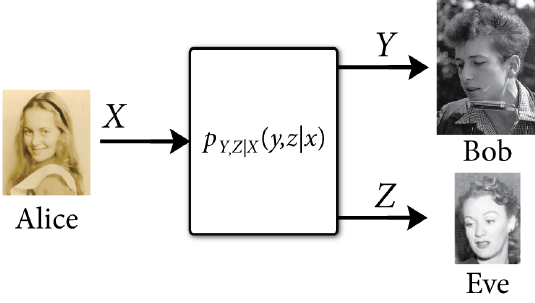
\includegraphics[width=0.6\textwidth]{figures/private_communication_wiretap_channel.png}
    \caption{Classical wiretap channel \cite{Wilde_2016}.}
\end{figure}

\subsection{Properties of Private Capacity of a Wiretap Channel}

\begin{theorem}[Non-negativity]
The private capacity $P(\mathcal{N})$ of a wiretap channel is non-negative.
$$P(\mathcal{N}) \geq 0$$
\end{theorem}

\begin{proof}
By setting the joint density $p_{U,X}(u, x)$ to the degenerate distribution $\delta_{u,u_0} \delta_{x,x_0}$ for specific values $u_0$ and $x_0$, both mutual information terms $I(U; Y)$ and $I(U; Z)$ become zero, resulting in a difference of zero. Since $P(\mathcal{N})$ involves a maximization over all possible distributions $p_{U,X}(u, x)$, the value of $P(\mathcal{N})$ cannot be negative.
\end{proof}

\begin{theorem}[Additivity]
Let $\mathcal{N}_i$ represent a classical wiretap channel given by $p_{Y_i, Z_i | X_i}$. The private capacity of the combined classical channel $\mathcal{N}_1 \otimes \mathcal{N}_2$ is given by the sum of the individual private capacities of $\mathcal{N}_1$ and $\mathcal{N}_2$.
$$P(\mathcal{N}_1 \otimes \mathcal{N}_2) = P(\mathcal{N}_1) + P(\mathcal{N}_2)$$
\end{theorem}

\begin{proof}
The inequality $P(\mathcal{N}_1 \otimes \mathcal{N}_2) \geq P(\mathcal{N}_1) + P(\mathcal{N}_2)$ follows from the fact that the two channels could be given by uncorrelated probability distributions. Since the maximization is over all possible probability distributions, the capacity would thus be atleast the throughput of the uncorrelated probability distributions, which is equal to the sum of the individual probability distributions.

In order to prove the reverse direction, we consider any probability distribution $p_{U, X_1, X_2}(u, x_1, x_2)$ for $P(\mathcal{N}_1 \otimes \mathcal{N}_2)$, where $X_1, X_2$ are the input random variables transmitted to the two channels. We can write the combined channel capacity as follows.

\begin{align*}
I(U; Y_1 Y_2) - I(U; Z_1 Z_2) &= I(U; Y_1) + I(U; Y_2 | Y_1) - I(U; Z_2) - I(U; Z_1 | Z_2) \\
&= I(U; Y_1 | Z_2) - I(U; Z_1 | Z_2) + I(U; Y_2 | Y_1) - I(U; Z_2 | Y_1)
\end{align*}

The first equality follows from the chain rule for mutual information, while the second follows from the following identity and some rearrangement of terms.
$$I(U; Y_1) - I(U; Z_2) = I(U; Y_1 | Z_2) - I(U; Z_2 | Y_1)$$

Consider the first two terms from the expanded form of combined channel capacity.

\begin{align*}
I(U; Y_1 | Z_2) - I(U; Z_1 | Z_2) &= \sum_{z_2} p_{Z_2}(z_2) [I(U; Y_1 | Z_2 = z_2) - I(U; Z_1 | Z_2 = z_2)] \\
&\leq \max_{z_2} [I(U; Y_1 | Z_2 = z_2) - I(U; Z_1 | Z_2 = z_2)] \\
&\leq P(\mathcal{N}_1)
\end{align*}

Similar argument yields the following relation.
$$I(U; Y_2 | Y_1) - I(U; Z_2 | Y_1) \leq P(\mathcal{N}_2)$$

Combining the two relations proves the other side of the inequality. The two inequalities together establish the additivity relation.
$$P(\mathcal{N}_1 \otimes \mathcal{N}_2) = P(\mathcal{N}_1) + P(\mathcal{N}_2)$$
\end{proof}

\begin{theorem}[Equivalence of asymptotic and single use capacity]
The asymptotic private capacity of a wiretap channel $\mathcal{N}$ is equal to its private capacity.
$$\lim_{n \rightarrow \infty} \frac{1}{n} P(\mathcal{N}^{\otimes n}) = P(\mathcal{N})$$
\end{theorem}

\begin{proof}
Consider the following inductive hypothesis for any positive value of $k$. It trivially holds for $k=1$.
\begin{align*}
P(\mathcal{N}^{\otimes k}) &= \sum_{i=1}^k P(\mathcal{N}) \\
&= k P(\mathcal{N}_i)
\end{align*}

Using the additivity relation and the inductive hypothesis, we can prove by induction that the hypothesis holds for $k+1$.
\begin{align*}
P(\mathcal{N}^{\otimes k} \otimes \mathcal{N}_{k+1}) &= P(\mathcal{N}^{\otimes k}) + P(\mathcal{N}_{k+1}) \\
&= \sum_{i=1}^{k} P(\mathcal{N}_i) + P(\mathcal{N}_{k+1}) \\
&= \sum_{i=1}^{k+1} P(\mathcal{N}_i) \\
&= (k+1) P(\mathcal{N})
\end{align*}

Moving the constant factor to the LHS and applying limits gives us the desired relation.
$$\lim_{n \rightarrow \infty} \frac{1}{n} P(\mathcal{N}^{\otimes n}) = P(\mathcal{N})$$
\end{proof}

\subsection{Private Capacity of a Quantum Channel}

Consider a quantum channel $\mathcal{N}$ given by the operator $\mathcal{U}_{A' \rightarrow BE}^{\mathcal{N}}$. In the private communication model, Alice would like to establish classical correlations with Bob, without the channel's environment of the channel having access to these correlations. Let the following be the density matrix of the classical-quantum state she transmits to the channel.

$$\rho_{XA'} = \sum_{x} p_X(x) \ket{x}\bra{x}_X \otimes \rho_{A'}^x $$

The private capacity $P(\mathcal{N})$ of a quantum channel $\mathcal{N}$ is defined similar to the private capacity of a wiretap channel. Here, we will replace the classical mutual information with quantum mutual information, and the maximization will be over all the classical quantum states described earlier.

\begin{definition}[Private Capacity of a Quantum Channel]
The private information $P(\mathcal{N})$ of a quantum channel $\mathcal{N}$ is defined as:
$$P(\mathcal{N}) = \max_{\rho_{XA'}} \left[ I(X;B)_\rho - I(X;E)_\rho \right]$$
\end{definition}

We shall see that this definition of private capacity too satisifies non-negativity, but in contrast to the case of wiretap channel it violates the additivity relation.

\begin{figure}[H]
    \centering
    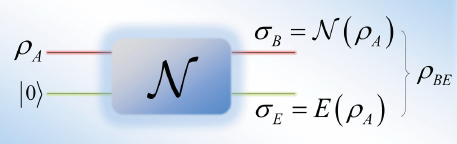
\includegraphics[width=0.6\textwidth]{figures/private_communication_quantum_channel.png}
    \caption{Private communication through a quantum channel \cite{Gyongyosi_2018}.}
\end{figure}

\subsection{Properties of Private Capacity of a Quantum Channel}

\begin{theorem}[Non-negativity]
The private capacity $P(\mathcal{N})$ of a quantum channel is non-negative.
$$P(\mathcal{N}) \geq 0$$
\end{theorem}

\begin{proof}
Similar to the proof in the classical wiretap channel case, we can consider a degenerate input state $\rho_{XA'}$ of the form $\ket{0}\bra{0}_X \otimes \psi_{A'}$, where $\psi_{A'}$ is a pure state. The private information of this state is zero. Since the maximization is over all possible input states, the private capacity of the channel is guaranteed to be atleast zero, or non-negative.
\end{proof}

\begin{theorem}[Additivity]
Let $\mathcal{N}_1$ and $\mathcal{N}_2$ represent two quantum channels. The private capacity of the combined quantum channel $\mathcal{N}_1 \otimes \mathcal{N}_2$ is not equal to the sum of the individual private capacities of $\mathcal{N}_1$ and $\mathcal{N}_2$.
$$P(\mathcal{N}_1 \otimes \mathcal{N}_2) \neq P(\mathcal{N}_1) + P(\mathcal{N}_2)$$
\end{theorem}

\begin{proof}
TODO
\end{proof}
